\documentclass{article}

% Language setting
% Replace `english' with e.g. `spanish' to change the document language
\usepackage[english]{babel}

% Set page size and margins
% Replace `letterpaper' with `a4paper' for UK/EU standard size
\usepackage[letterpaper,top=2cm,bottom=2cm,left=3cm,right=3cm,marginparwidth=1.75cm]{geometry}

% Useful packages
\usepackage{amsmath}
\usepackage{authblk}
\usepackage{lmodern}
\usepackage{graphicx}
\usepackage{todonotes}
\usepackage{placeins}   % helps to keeps figures at the same page or within the /FloatBarrier
\usepackage{caption}    % lets you define the fontsize of figure captions
\usepackage[colorlinks=true, allcolors=blue]{hyperref}

\renewcommand\Authfont{\fontsize{9}{10}\selectfont}
\renewcommand\Affilfont{\fontsize{8}{9}\itshape}

\title{Implementation of an On-Board Terrain Classifier based on Proprioceptive Sensor Data for a Planetary Rover}
\author[1]{Raul Dominguez}
\author[2]{Lennart Kuhr}
\author[1]{Jonathan Babel}
\author[1]{Florian Cordes}
\author[3]{Giulio Reina}
\author[1,4]{Frank Kirchner}
\affil[1]{DFKI Robotics Innovation Center Bremen Robert-Hooke-Str. 1, 28359 Bremen, Germany, \newline E-mail: name.surname@dfki.de}
\affil[2]{Institute of Space Systems, TU Braunschweig, Herman-Blenck-Straße 23, 38108 Braunschweig, Germany, \newline E-mail: l.kuhr@tu-braunschweig.de}
\affil[3]{Department of Mechanics, Mathematics and Management, Polytechnic of Bari, Via Orabona 4, 70125, Bari, Italy, E-mail: giulio.reina@poliba.it}
\affil[4]{Robotics Research Group, University of Bremen, Germany}

\begin{document}

\date{}
\maketitle
\captionsetup[figure]{font=footnotesize}

%\begin{abstract}

%\end{abstract}

%\section{Introduction}

% Introduction main motivation and main idea of the paper explain in detail the implementation of a SMV-based proprioceptive terrain classifier
Planetary explorations missions are so far dominated by wheeled rover designs like Curiosity
or Perseverance \cite{moeller2021, welch2013}. Although wheeled locomotion is most energy-efficient
over flat terrain, it compromises drawbacks when exposed to demanding unstructured
terrain. Especially in unstructured environments with steep, sandy slopes and boulders
patches, wheeled systems reach their limitations \cite{kolvenbach2021}. In the past, several high slip and
excessive sinkage events have been encountered with exploration rovers, which have severely
disrupted the mission timeline \cite{gonzalez2018}. For example, it took five weeks to free the Opportunity
rover from sand in 2006 \cite{young2006}, and rover trajectories are frequently adjusted to avoid
challenging terrain \cite{arvidson2017}. The potentially worst situation occurred in 2009 when the
Spirit rover got stuck in the sand and was unable to recover, ultimately ending the mission
\cite{webster2009}. 
Terrain awareness, the correct modeling of the surfaces transited and its classification is a key factor for reliable autonomous navigation and environment modelling. 
An appropriate surface modelling can be used to avoid rover navigation operations problems as the ones described before. 
Moreover, terrain awareness can be used to enhance navigation capabilities by adapting system settings in accordance to the terrain properties.

In this publication a software component implementation capable of classifying the traversed terrain type based on proprioceptive sensor data is presented. 
The component uses a Support Vector Machine (SVM) algorithm \cite{vapnik1992,cristianini2000} in its core. It is integrated into the software control architecture of the mobile exploration robot SherpaTT, such that it can be executed sufficiently fast during navigation. SherpaTT is a hybrid wheeled-leg rover with an actively articulated suspension system. Its locomotion control system provides the basis for advanced locomotive capabilities with the ability to adapt to different terrain types \cite{cordes2018}. 
The novel software component has been implemented using the framework Robotic Construction Toolkit (Rock)\footnote{Rock: The Robot Construction Kit (\url{http://rock-robotics.org})}. The diagram in Figure~\ref{fig:overview} presents the implementation approach of the terrain classifier in Rock.

% Challenges
One of the main challenges addressed by the middleware component is to generate matrices of synchronous sample values for classification online from datastreams with multiple frequencies.
%During the traverse the terrain classifier component uses proprioceptive sensor data -force torque sensors and joints- and dataproducts -acceleration estimates- to classify between the three terrain types.
% Background and approach
During navigation the terrain classifier uses force torque sensors, joint data and body acceleration estimates to classify the surface into one of three terrain types: \emph{sand, compact sand} and \emph{concrete}.
The three types represent distinct classes of surfaces characterized by its deformability and friction properties, but are hard to identify with exteroceptive sensors since they are visually similar.
In order to achieve a better classification performance as well as a more in-depth characterization of the surface patches, a feature calculation process is performed. 
The computed features estimate physical properties such as mechanical power, electrical power, friction coefficients and speed deviation. Along with all of these features, the corresponding statistical values, i.e. variance, skewness and kurtosis are evaluated. 
Finally, critical features for terrain classification must be identified to reduce the dimensionality of inputs to the classifier.
This feature selection process was done using a WB index and the Pearson Coefficient as detailled in \cite{Dimastrogiovanni2020}. 
Furthermore, the classification results need to be available at a fast enough pace to allow other onboard components take advatange of the results (e.g. to improve navigation) and to ensure that the classification results correspond to the currently traversed surface. 
Likewise, the loss of data samples due to full queues on the input of the processing components must be avoided. 


\begin{figure}
\centering
\includegraphics[width=\textwidth]{../figures/OverviewTC2.pdf}
\caption{\label{fig:overview}Overiview of the terrain classifier library and Rock integration.}
\end{figure}

\begin{figure}[b!]
\centering
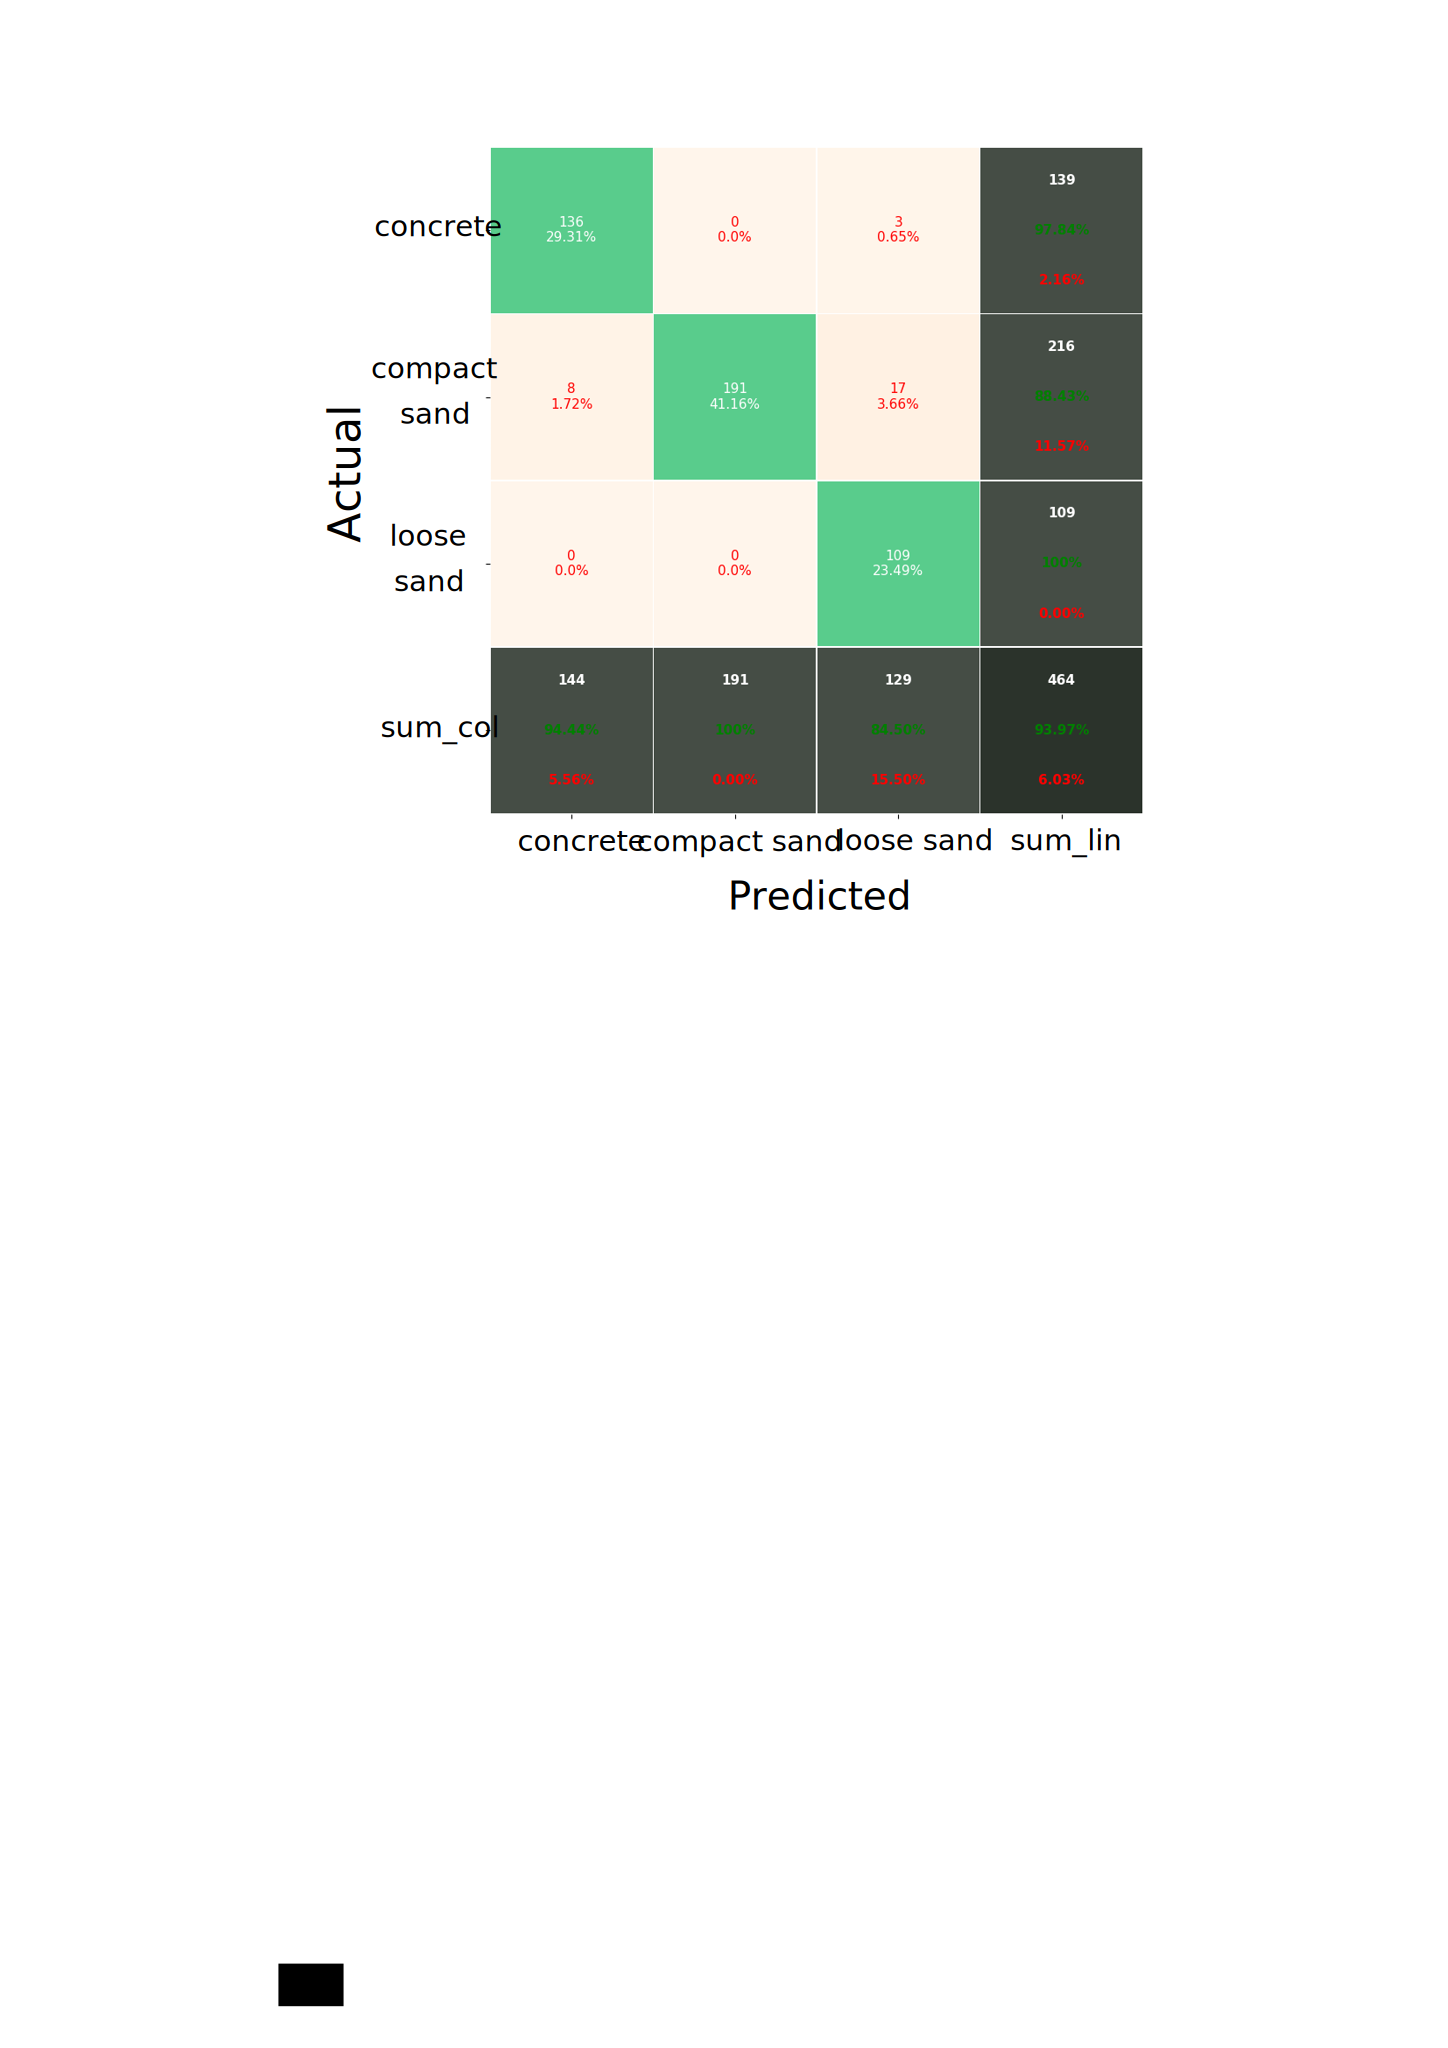
\includegraphics[width=0.5\textwidth]{../figures/confusionmatrix_Train.png}
\caption{\label{fig:confusionmatrix} Shows the performance of the SVM model. Except the recall for \emph{compact sand} and the precision for \emph{sand} all performances are above 90\%, with an overall accuracy of 93.97\%}
\end{figure}

% The SVM model training software is implemented to enable the use of a variable constellation of logged datasets. Moreover, it can be used to compare both the offline and online classification performance. 

% Evaluation
The initial offline evaluation of the SVM classifier reached an accuracy of 93.97\% as shown in the confusion matrix in Figure~\ref{fig:confusionmatrix}.
Results generated from several test traverses of SherpaTT were logged to analyze the onboard classification performance and compared with the ones obtained from training sets. A complete analysis of performance was not possible, because the traversed terrain during the field tests did not closly match the previously trained terrain classes. Nevertheless, the software shows good classification results, since the type of surface -\emph{wet compact sand}- was close to the two classes mostly identified -\emph{concrete} and \emph{compact sand}.
Several field tests demonstrated that the terrain classifier can be executed on SherpaTT and that it is able to compute features as well as classify different terrain types succesfully, whilst the rover is traversing the surface. The C++ calculations and terrain classifications were executed in sufficient time in parallel to the rest of SherpaTT's Motion Control System, on a single thread, using a i7 processor with a CPU clock speed of 4.6 GHz. 


%Moreover, the classification performance achieved onboard SherpaTT was identified during tests on terrain that represent at least one of the three terrain type classes.

\FloatBarrier

\bibliographystyle{alpha}
\bibliography{sample}

\end{document}
